% !TeX root = ../Book2.tex
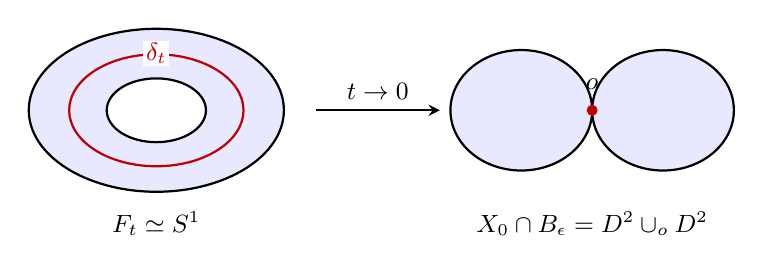
\begin{tikzpicture}[scale=.9,>=stealth, every node/.style={font=\small}]
	\fill[blue!9,even odd rule] (0,0) ellipse (1.8 and 1.15) (0,0) ellipse (.7 and .45);
	\draw[thick] (0,0) ellipse (1.8 and 1.15);
	\draw[thick] (0,0) ellipse (.7 and .45);
	\draw[red!75!black,thick] (0,0) ellipse (1.23 and .79);
	\node[red!75!black,fill=white,inner sep=1pt] at (0,.8) {$\delta_t$};
	\node at (0,-1.6) {$F_t\simeq S^1$};
	\draw[->,thick] (2.25,0)--(4,0) node[midway,above] {$t\to0$};
	\fill[blue!9] (5.15,0) ellipse (1 and .85);
	\fill[blue!9] (7.15,0) ellipse (1 and .85);
	\draw[thick] (5.15,0) ellipse (1 and .85);
	\draw[thick] (7.15,0) ellipse (1 and .85);
	\fill[red!75!black] (6.15,0) circle (2.2pt);
	\node[above=4pt] at (6.15,0) {$o$};
	\node at (6.15,-1.6) {$X_0\cap B_\epsilon=D^2\cup_oD^2$};
\end{tikzpicture}
